\documentclass[12pt,letterpaper]{book}
\usepackage{mathptmx}
\usepackage[latin1]{inputenc}
\usepackage[spanish,es-tabla]{babel}
\usepackage{amsmath}
\usepackage{amssymb, amsfonts, latexsym, cancel}
\usepackage{transparent}
\usepackage{eso-pic,graphicx}
\usepackage{epstopdf}
\usepackage{float}
\usepackage{subfigure}
\usepackage{array}
\usepackage{longtable}
\usepackage[left=2cm,right=2cm,top=2cm,bottom=2cm]{geometry}
\usepackage{bm}
\usepackage{appendix}
\usepackage{subfigure}
\usepackage[subfigure]{tocloft}
\usepackage{multirow} % para las tablas
\usepackage{longtable}
\usepackage{lipsum}
\usepackage[breaklinks=true]{hyperref}
\usepackage[acronym,section=section]{glossaries}
\usepackage{fancyhdr, lastpage}
\usepackage{afterpage}
\usepackage{caption,newfloat}
%%%%%%%%%%%%%%%%%%%%%%%%%%%%%%%%%%%%%%%%%%%%%%%%%%
% Agregar una pagina en blanco
\newcommand\blankpage{%
    \null
    \thispagestyle{empty}%
    \addtocounter{page}{-1}%
    \newpage}
%%%%%%%%%%%%%%%%%%%%%%%%%%%%%%%%%%%%%%%%%%%%%%%%%%
% Modificacion de estilos de encabezados y pie de pagina
\fancypagestyle{plain}{
  \fancyhf{}% Clear header/footer
  \fancyfoot[R]{\thepage}% Right footer
  \renewcommand{\headrulewidth}{0.0pt}%
}
\pagestyle{plain}% Set page style to plain.
%%%%%%%%%%%%%%%%%%%%%%%%%%%%%%%%%%%%%%%%%%%%%%%%%%
% Modificar los niveles de nuemeracion
\setcounter{secnumdepth}{4}
%%%%%%%%%%%%%%%%%%%%%%%%%%%%%%%%%%%%%%%%%%%%%%%%%%
% Modificacion de sangria
\parindent=0cm 
%%%%%%%%%%%%%%%%%%%%%%%%%%%%%%%%%%%%%%%%%%%%%%%%%%
% configuracion de anexos
\renewcommand{\appendixname}{Anexos}
\renewcommand{\appendixtocname}{Anexos}
\renewcommand{\appendixpagename}{Anexos}
\begin{document}
\frontmatter
\begin{titlepage}
\begin{center}
\AddToShipoutPictureBG*{\transparent{0.25}
\includegraphics[width=\paperwidth,height=\paperheight]{graphics/logo.jpg}}
{\LARGE \textbf{UNIVERSIDAD RAFAEL LAND\'IVAR}}\\[0.1cm]
{\normalsize FACULTAD DE INGENIER\'IA}\\[0.1cm]
{\normalsize DEPARTAMENTO DE INGENIER\'IA EN INFORM\'ATICA Y SISTEMAS}\\[4cm]
{\huge \textbf{Aplicaci\'on del algoritmo de Random Forest Regression para la detecci\'on de los pasos requeridos de un movimiento v\'alido mediante la utilizaci\'on del dispositivo Kinect V2}}\\[0.1cm]
{\LARGE PROYECTO DE INGENIER\'IA}
\vfill
DIEGO JOS\'E ORELLANA BOJORQUEZ\\[0.1cm]
CARN\'E 10101-14\\[2cm]
Guatemala, Enero de 2020\\[0.1cm]
Campus Central
\afterpage{\blankpage}
\end{center}
\end{titlepage}
\begin{center}
\AddToShipoutPictureBG*{\transparent{0.25}
\includegraphics[width=\paperwidth,height=\paperheight]{graphics/logo.jpg}}
{\LARGE \textbf{UNIVERSIDAD RAFAEL LAND\'IVAR}}\\[0.1cm]
{\normalsize FACULTAD DE INGENIER\'IA}\\[0.1cm]
{\normalsize DEPARTAMENTO DE INGENIER\'IA EN INFORM\'ATICA Y SISTEMAS}\\[4cm]
{\huge \textbf{Aplicaci\'on del algoritmo de Random Forest Regression para la detecci\'on de los pasos requeridos de un movimiento v\'alido mediante la utilizaci\'on del dispositivo Kinect V2.}}\\[0.1cm]
{\LARGE PROYECTO DE INGENIER\'IA}
\vfill
{\LARGE Presentada ante el Consejo de la Facultad de Ingenier\'ia}
\vfill
{\LARGE Por:}\\[0.1cm]
{\LARGE \textbf{DIEGO JOS\'E ORELLANA BOJORQUEZ}}
\vfill
Previo a optar el t\'itulo de:\\[0.1cm]
Ingeniero en Inform\'atica y Sistemas
\vfill
En el grado acad\'emico de:\\[0.1cm]
Licenciado
\vfill
Guatemala, Enero de 2020\\[0.1cm]
Campus Central
\end{center}
%%%%%%%%%%%%%%%%%%%%%%%%%%%%%%%%%%%%%%%%%%%%%%%%%
% notificaci�n
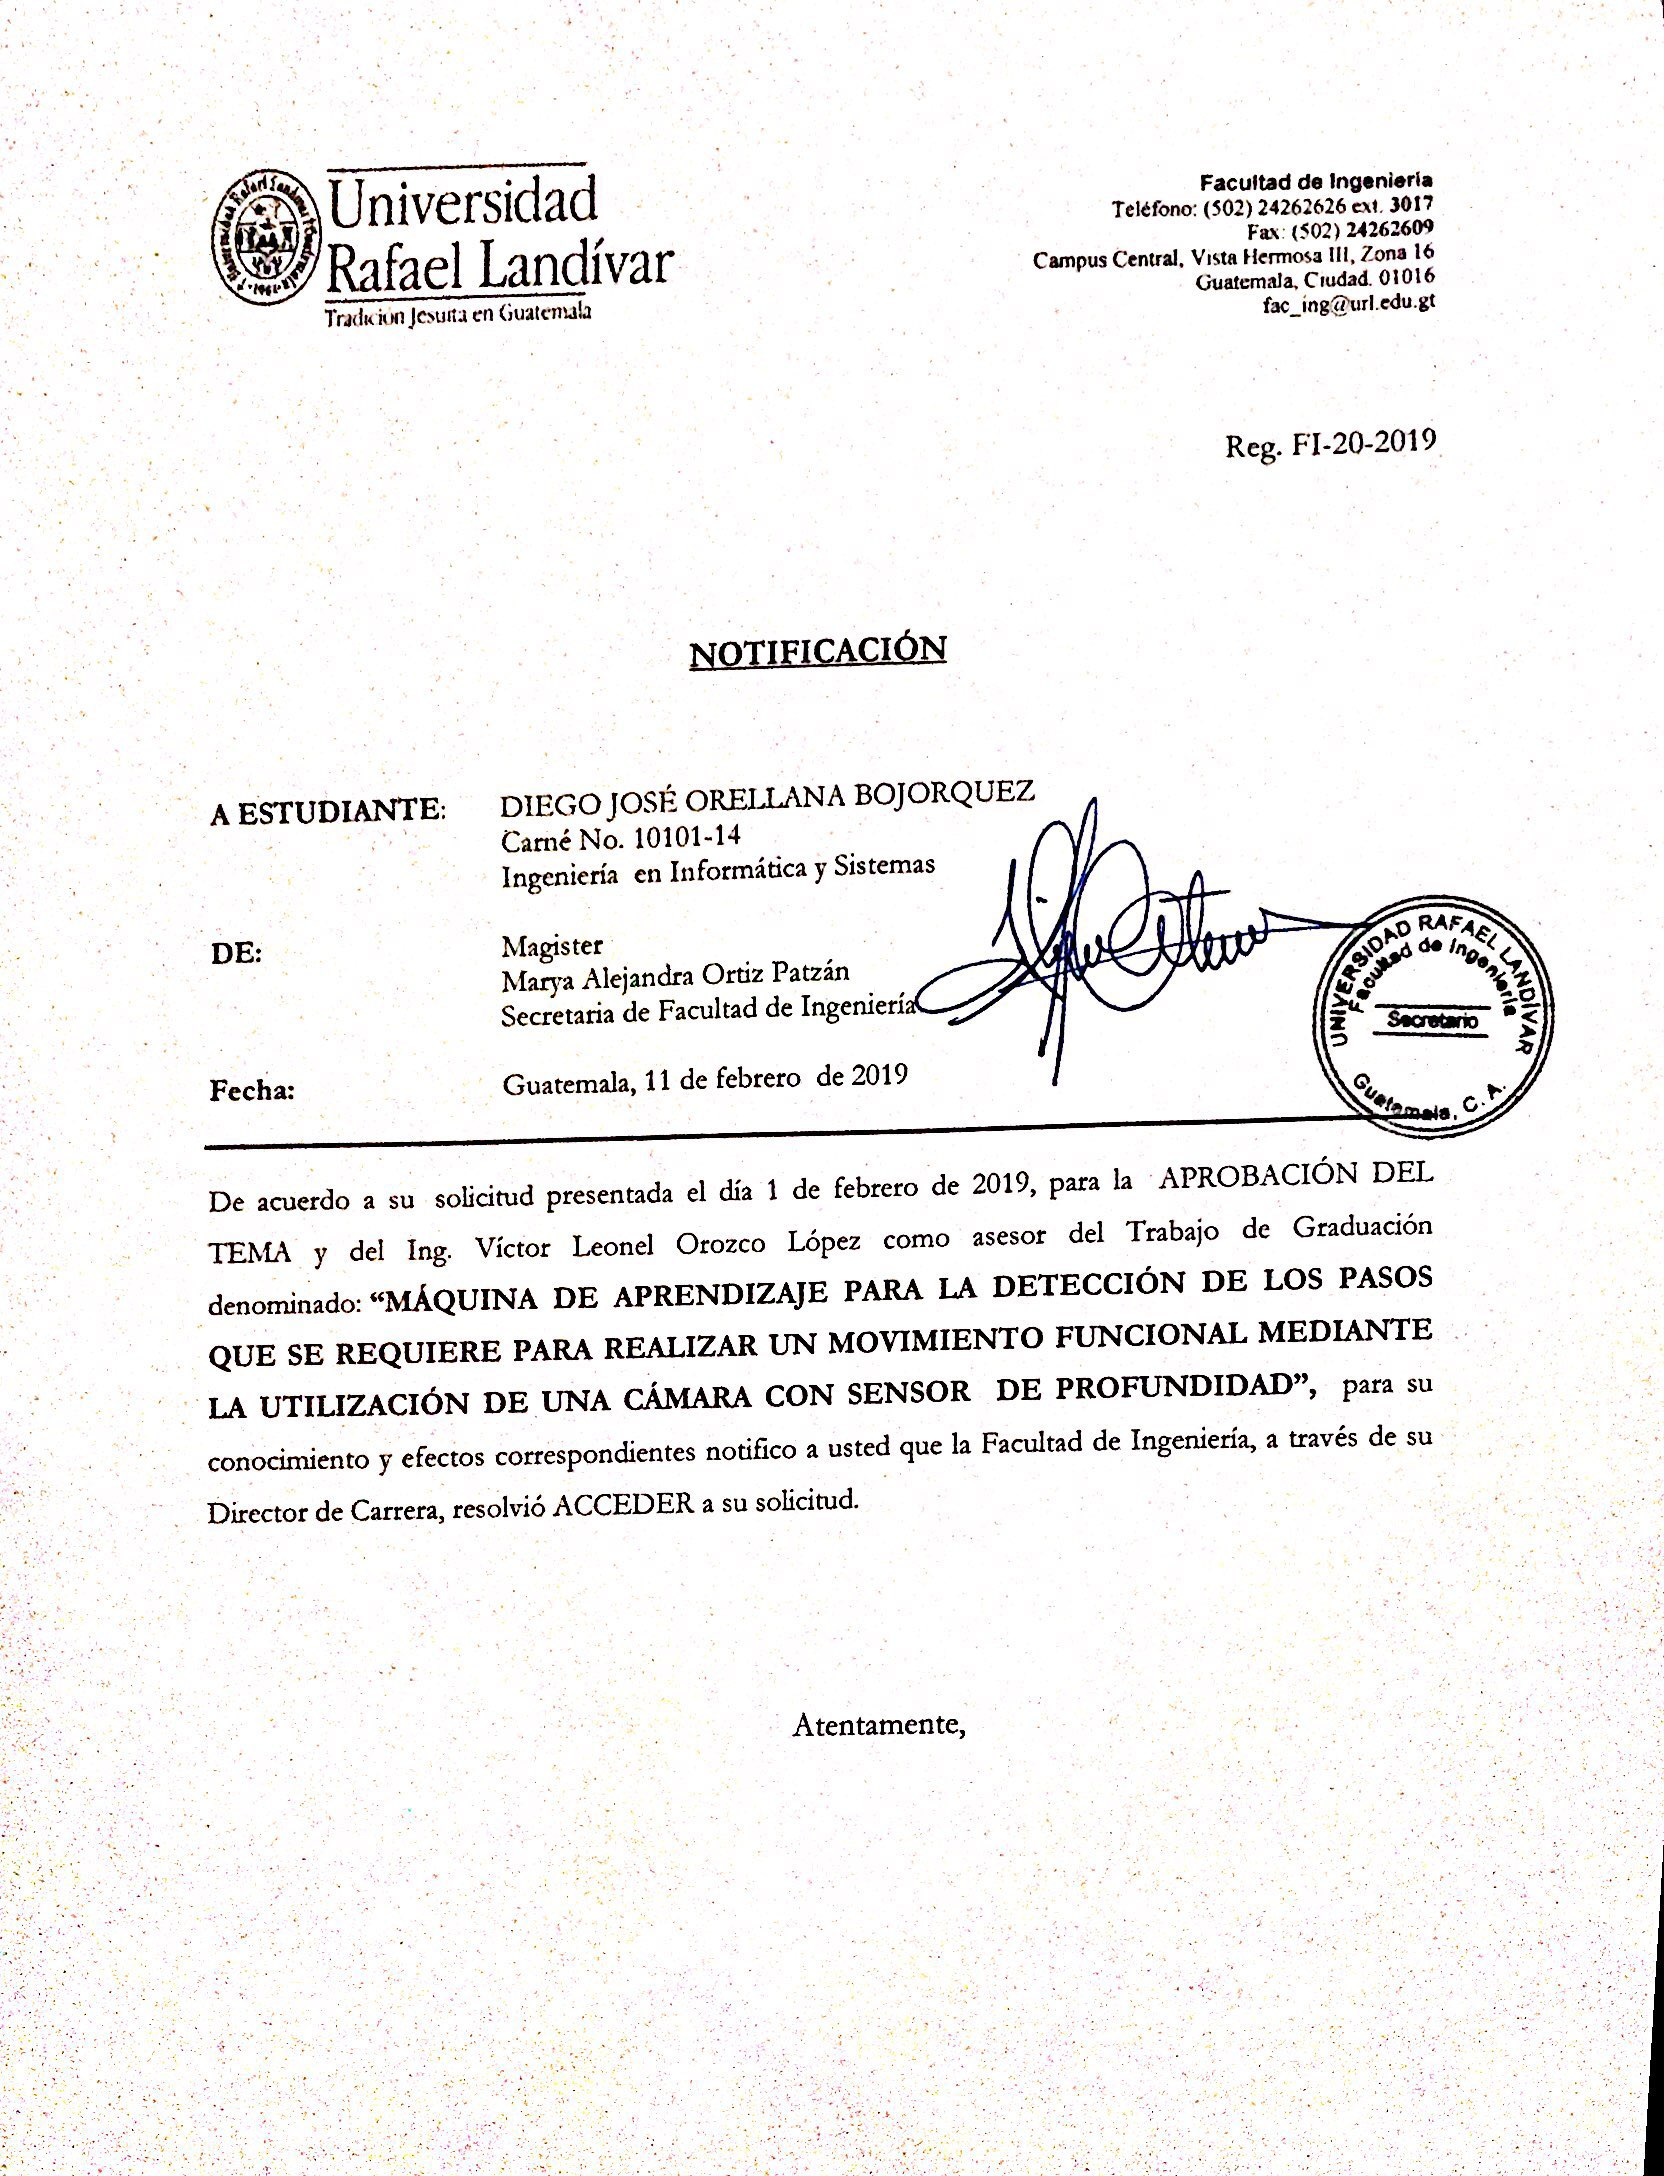
\includegraphics[width=18cm,height=22cm]{graphics/notificacion-tesis.jpg}
%%%%%%%%%%%%%%%%%%%%%%%%%%%%%%%%%%%%%%%%%%%%%%%%%
\afterpage{\blankpage}
\newpage
{\LARGE \textbf{Agradecimientos}}\\[2cm]
\begin{itemize}
\item A Dios, por ser alguien que me escucha en todo momento.
\item A mi mam\'a, gracias a ella he llegado tan lejos, adem\'as de estar siempre conmigo en las buenas y en las malas. 
\item A mi hermanos, por tenerme paciencia y confiar en m\'i en todo momento.
\item A mi pap\'a, por acompa\~narme siempre.
\item A mis amigos de la universidad, por ser una gran promoci\'on unida y apoyarnos en todo momento.
\item A mis amigos del colegio, por mantener nuestra amistad y vernos crecer.
\item Ingenieros Stanly Bola\~nos y Victor Orozco, por apoyarme en todo el proceso de trabajo de investigaci\'on.
\item Departamento de deportes de la universidad Rafael Land\'ivar, por confiar en mi proyecto de ingenier\'ia.
\end{itemize}
\begin{center}
Diego Orellana.
\end{center}
\afterpage{\blankpage}
\newpage
\tableofcontents.
\listoffigures.
\listoftables.
\listofcharts.
\listofformulas.
\listofcodes.
\mainmatter
%index
\chapter{INTRODUCCI�N}
\section{LO ESCRITO SOBRE EL TEMA}
\section{MARCO TE�RICO}
\chapter{PLANTEAMIENTO DEL PROBLEMA}
\section{OBJETIVOS}
\subsection{OBJETIVO GENERAL}
\subsection{OBJETIVOS ESPEC�FICOS}
\section{HIP�TESIS}
\section{VARIABLES}
\subsection{VARIABLES DEPENDIENTES}
\subsection{VARIABLES INDEPENDIENTES}
\section{DEFINICI�N DE LAS VARIABLES}
\subsection{DEFINICI�N CONCEPTUAL}
\subsection{DEFINICI�N OPERACIONAL}
\section{ALCANCES}
\section{L�MITES}
\section{APORTE}
\chapter{M�TODO}
\section{SUJETOS}
\subsection{PRIMER TIPO}
\subsection{SEGUNDO TIPO}
\section{UNIDADES DE AN�LISIS}
\section{INSTRUMENTOS}
\section{PROCEDIMIENTO}
\section{DISE�O Y METODOLOG�A ESTAD�STICA}
\subsection{DISE�O EXPERIMENTAL}
\subsubsection{EXPERIMENTOS}
\subsubsection{TRATAMIENTOS Y REPETICIONES EN LOS EXPERIMENTOS}
\chapter{PRESENTACI�N Y AN�LISIS DE RESULTADOS}
\chapter{DISCUSI�N}
\chapter{CONCLUSIONES}
\chapter{RECOMENDACIONES}
\backmatter
\chapter{REFERENCIAS BIBLIOGR�FICAS}
\appendix
\clearpage
\addappheadtotoc
\appendixpage

\end{document}